\section{Rilevamento movimento del dispositivo}
Qualora venga abilitato l'utilizzo dell'accelerometro, l'applicazione monitorerà lo stato del dispositivo studiando l'evoluzione delle informazioni ottenute tramite l'accelerometro e le interpreterà a seconda della sensibilità impostata dall'utente tramite la schermata iniziale.\\

L'accelerometro fornisce all'applicazione tre valori corrispondenti alle accelerazioni subite dal dispositivo sui tre assi X, Y e Z.
\begin{figure}[!ht]
\begin{center}
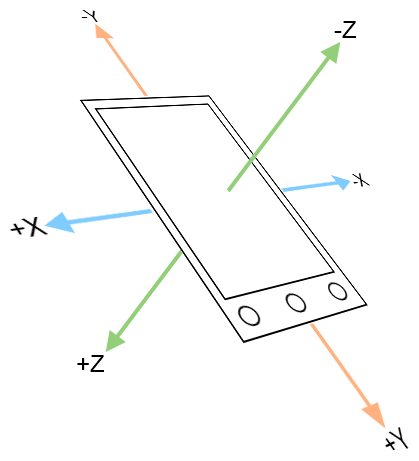
\includegraphics[scale=.5]{./../wireless/resources/accelerometer.png}
\caption{Verso delle accelerazioni determinate dall'accelerometro.}
\label{fig:Accelerometro}
\end{center}
\end{figure}
L'applicazione utilizza questa tripla di valori per ottenere una stima del movimento subito dal dispositivo. Poiché una sola tripla di valori permette solamente di determinare l'orientamento del dispositivo e non l'intensità con cui è mosso, è necessario campionare tali valori per un dato periodo di tempo e determinare se durante tale periodo l'orientamento del dispositivo ha registrato variazioni significative da poter essere tradotte in un movimento del dispositivo stesso.\\
La stima del movimento avviene utilizzando la formula:
\[variation = \frac{(\Delta accel_X) + (\Delta accel_Y) + (\Delta accel_Z)}{\Delta t}\]
Per determinare se il movimento è riconducibile ad uno stato anormale del dispositivo (si presume che il movimento sia conseguenza di un'avvenuta invasione), la stima del movimento viene in seguito confrontata con la soglia di sensibilità impostata dall'utente:
\begin{itemize}
  \item \texttt{LOW}: determina l'avvenuta intrusione qualora $variation >  3100$
  \item \texttt{MEDIUM}: determina l'avvenuta intrusione qualora $variation > 2700$
  \item \texttt{HIGH}: determina l'avvenuta intrusione qualora $variation > 2300$
\end{itemize}~\\

La tripla di informazioni ottenuta dall'accelerometro viene inoltre utilizzata per eseguire un display grafico dell'orientamento del dispositivo stesso. Viene animata una superficie tridimensionale (che rappresenta il dispositivo) e viene ruotata a seconda dell'effettivo orientamento calcolato dall'accelerometro. Per fornire questa rappresentazione animata tridimensionale si sfruttano le API OpenGL ES di modo da poter utilizzare la GPU e non appesantire la CPU di ulteriori calcoli.
\begin{figure}[!ht]
\begin{center}
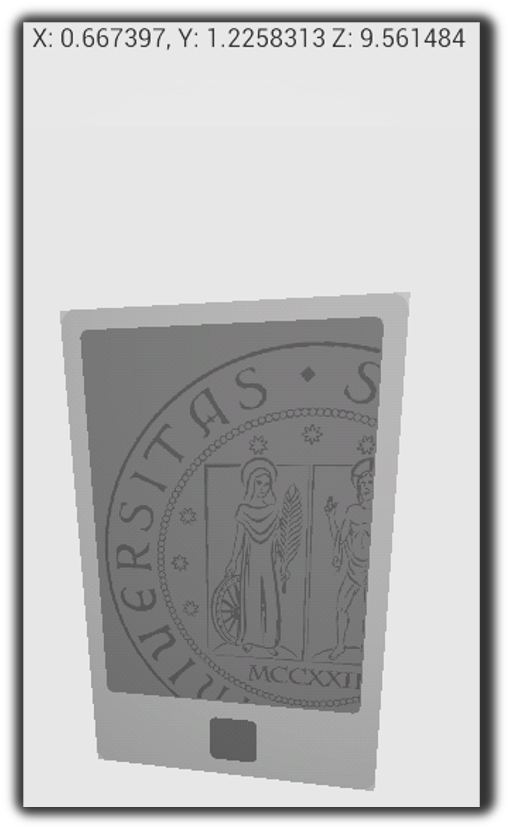
\includegraphics[scale=.3]{./../wireless/resources/opengl.png}
\caption{Display grafico dell'orientamento del dispositivo.}
\label{fig:OpenGL}
\end{center}
\end{figure}
